\documentclass[11pt, openright, a4paper, brazil, english, french, spanish, bibjustif, openany, oneside]{abntex2}

%template do beamer
%\usetheme{Feather}

\usepackage{cmap}				% Mapear caracteres especiais no PDF
\usepackage{ifthen}				% Mapear caracteres especiais no PDF
\usepackage{setspace}				% Mapear caracteres especiais no PDF
\usepackage{lmodern}		
\usepackage[T1]{fontenc}	
\usepackage[utf8]{inputenc}
\usepackage{lastpage}
\usepackage{enumitem}	
\usepackage{indentfirst}	
\usepackage{color}			
\usepackage{graphicx}
\usepackage[table]{xcolor}
\usepackage{tabularx}
\usepackage{booktabs}
\usepackage{enumerate}		
\usepackage{microtype} 		
\usepackage{multicol}
\usepackage{multirow}
\usepackage{lipsum}
\usepackage{booktabs}				
\usepackage{bold-extra}				% Mapear caracteres especiais no PDF
\usepackage[final]{pdfpages}
\usepackage{float}

%pacote para símbolos especiais
\usepackage{amssymb}

%pacote para fazer diagramas de venn

\usepackage{venndiagram}

%aumentei para fazer texto em fundo colorido
\usepackage{xcolor}
%aumentei a próxima linha
\usepackage{verbatim}

% \usepackage{subfig}
\usepackage{subcaption}


\usepackage[brazilian,hyperpageref]{backref}	 % Paginas com as citações na bibl
\usepackage[alf]{abntex2cite}	% Citações padrão ABNT

\usepackage{caption}


\newtheorem{teo}{Teorema}

%espaçamento do parágrafo
	 
\setlength{\parskip}{0.2cm}


\begin{document}


\begin{SingleSpace}


\begin{comment}

Quando quiser usar fundos coloridos

\colorbox{green}
{
\begin{minipage}{14.7cm}



\end{minipage}
}

Quando quiser usar textos ao lado um do outro ou figuras ao lado de textos

\begin{minipage}{.6\linewidth}

\end{minipage}

\end{comment}




\selectlanguage{brazil}


\frenchspacing 

%\ABNTEXchapterfont



\chapter*{Conjuntos Numéricos}

\section*{Introdução}

Como o próprio nome indica, toda coleção de objetos, pessoas, animais ou coisas constitui um \textbf{conjunto}. Os objetos que formam um conjunto são denominados \textbf{elementos}. Os elementos de um conjunto são indicados por letras minúsculas \textbf{a, b, c, ...} e os conjuntos, por letras maiúsculas \textbf{A, B, C, ...}.

Alguns termos e definições são importantes para o nosso estudo dos conjuntos:

\begin{itemize}

\item \textbf{Pertinência}

\colorbox{green}
{
\begin{minipage}{14.7cm}

Um elemento pode pertencer ou não pertencer a um determinado conjunto. Para indicar que um elemento pertence a um dado conjunto, utilizamos o símbolo \textcolor{red}{$\in$} e quando não pertence usamos o \textcolor{red}{$\not\in$}.

\textbf{Exemplos}:

$x \in A$ (Lê-se: $x$ pertence a $A$)

$x \not\in B$ (Lê-se: $x$ não pertence a $B$) 

\end{minipage}
}

\textbf{Observação}: Os símbolos $\in$ e $\not\in$ são utilizados para relacionar elemento com conjunto.

\item \textbf{Igualdade de conjuntos}

\colorbox{green}
{
\begin{minipage}{14.7cm}

Dois conjuntos são iguais quando possuem os mesmos elementos.

Indica-se: $A=B$

\end{minipage}
}


\item \textbf{Conjunto vazio}

\colorbox{green}
{
\begin{minipage}{14.7cm}

Conjunto vazio é o conjunto que não possui elementos.

Representa-se o conjunto vazio por $\textcolor{red}{\{\}}$ ou $\textcolor{red}{\emptyset}$.


\end{minipage}
}


\item \textbf{Conjunto universo}

\colorbox{green}
{
\begin{minipage}{14.7cm}

Conjunto universo é o conjunto ao qual pertencem os elementos de todos os conjuntos que fazem parte do nosso estudo.

\end{minipage}
}

\item \textbf{subconjuntos}

\colorbox{green}
{
\begin{minipage}{14.7cm}

Dados dois conjuntos, $A$ e $B$, dizemos que $A$ é subconjunto de $B$ se cada elemento do conjunto $A$ é, também, elemento do conjunto $B$.

Indicamos essa relação por:

\begin{center}

$A \subset B$ (Lê-se: $A$ está contido em $B$)

\end{center}

Ou também por:

\begin{center}

$B \supset A$ (Lê-se: $B$ contém $A$).

\end{center}

\end{minipage}
}

\textbf{Observações:}

      \begin{enumerate}[label=\textbf{\arabic*\textsuperscript{\d a})}]
      
      \item Escreveremos $A \not\subset B$ ($A$ não está contido em $B$) ou $B \not\supset A$ ($B$ não contém $A$), se $A$ não for subconjunto de $B$.
      
      \item Os símbolos $\subset$, $\not\subset$, $\supset$ e $\not\supset$ são utilizados para relacionar conjunto com conjunto.
      
      \end{enumerate}
      
    

\end{itemize}


\section*{Como representar um conjunto}

Um conjunto pode ser representado de três formas:

\begin{itemize}

\item \textbf{1\textsuperscript{\d a} forma}: por extensão

\end{itemize}

Enumeram-se seus elementos, escrevendo-os entre chaves e separando-os por vírgulas. Por exemplo, o conjunto dos dias da semana:

$A=\{$domingo, segunda-feira, terça-feira, quarta-feira, quinta-feira, sexta-feira, sábado$\}$.

Podemos também utilizar a representação por extensão mesmo que o conjunto seja \textbf{infinito} ou seja \textbf{finito} mas com um número elevado de elementos.

\textbf{Exemplos}: 



\begin{enumerate}[label=\alph*)]

\item Conjunto dos números pares:

$A=\{$ 2, 4, 6, ...$\}$ $\rightarrow$ Conjunto infinito

\item Conjunto dos números naturais menores que 500:

$B=\{$ 0, 1, 2, 3, ..., 499 $\}\rightarrow$ Conjunto finito

\end{enumerate}

\begin{itemize}

\item \textbf{2\textsuperscript{\d a} forma}: por compreensão

\end{itemize}

O conjunto será representado por meio de uma propriedade que caracteriza os seus elementos.

\textbf{Exemplos}: a) $A=\{ x \mid x \in \mathbb{Z}$ e $ x < 8\}$ \hspace{2cm} b) $B=\{ x \mid x$ é vogal$\}$

Observe que a propriedade que caracteriza o conjunto permite estabelecer se um dado elemento pertence ou não ao conjunto.

\begin{itemize}

\item \textbf{2\textsuperscript{\d a} forma}: por figuras

\end{itemize}

Toda figura utilizada para representar um conjunto é chamada de \textbf{diagrama de Venn}. Por exemplo, o conjunto $A=\{1, 2, 3, 4\}$ pode ser representado pelo diagrama:

\begin{minipage}{.4\linewidth}

\begin{figure}[H]
    
    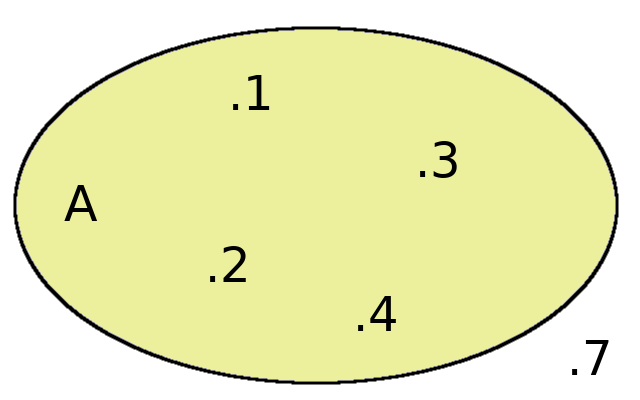
\includegraphics[width=3cm]{diagramadevenn1.png}
   
\end{figure} 

\end{minipage}
\begin{minipage}{.6\linewidth}

Os elementos de $A$ são representados por pontos internos desta figura. Observe que $2 \in A$ (é um ponto interno) e $7 \not\in B$ (é um ponto externo)

\end{minipage}

\vspace{1cm}

\section*{Operações com conjuntos}

\vspace{.5cm}

\begin{itemize}

\item \textbf{\resizebox{!}{.4cm}{União de conjuntos}}

\end{itemize}

Sejam os conjuntos $A=\{0, 2, 4, 6\}$ e $B=\{0, 1, 2, 3, 4\}$. Vamos determinar um conjunto $C$ formado pelos elementos que pertencem a $A$ ou a $B$ ou a ambos:

\begin{center}
\begin{minipage}{.3\linewidth}

\begin{flushright}

$A=\{0, 2, 4, 6\}$

$B=\{0, 1, 2, 3, 4\}$

\end{flushright}

\end{minipage}
\begin{minipage}{.2\linewidth}

\resizebox{3cm}{.4cm}{$\Rightarrow$}

\end{minipage}
\begin{minipage}{.3\linewidth}

\begin{flushleft}

$C=\{0, 1, 2, 3, 4, 6\}$

\end{flushleft}

\end{minipage}

\end{center}

O conjunto $C$ assim formado, é chamado \textbf{união} de $A$ e $B$.

Então:

\colorbox{green}
{
\begin{minipage}{14.7cm}

A união de dois conjuntos, $A$ e $B$, é o conjunto formado por todos os elementos que pertencem a $A$ ou a $B$.
Designamos a união de $A$ e $B$ por $A \cup B$ (lê-se: $A$ união $B$).

$A \cup B=\{x \mid x \in A$ ou $x \in B\}$

\end{minipage}
}

Exemplos:

\begin{enumerate}[label=\alph*)]

\item $A=\{0, 1, 2, 3, 4\}$, $B=\{1, 3, 5, 7\} \Rightarrow A \cup B=\{0, 1, 2, 3, 4, 5, 7\}$

\item $A=\{0, 1, 2\}$, $B=\{ 0, 1, 2, 3, 4\} \Rightarrow A \cup B=\{0, 1, 2, 3, 4\}$

\item $A=\{0, 2\}$, $B=\{1, 3, 5\} \Rightarrow A \cup B=\{0, 1, 2, 3, 5\}$

\end{enumerate}

\vspace{.5cm}

\begin{itemize}

\item \textbf{\resizebox{!}{.4cm}{Intersecção de conjuntos}}

\end{itemize}

Sejam os conjuntos $A=\{0, 2, 4, 6\}$ e $B=\{0, 1, 2, 3, 4\}$.
Vamos determinar um conjunto $C$ formado pelos elementos que são comuns a $A$ e a $B$, ou seja, pelos elementos que pertencem a $A$ e também pertencem a $B$:


\begin{center}
\begin{minipage}{.3\linewidth}

\begin{flushright}

$A=\{0, 2, 4, 6\}$

$B=\{0, 1, 2, 3, 4\}$

\end{flushright}

\end{minipage}
\begin{minipage}{.2\linewidth}

\resizebox{3cm}{.4cm}{$\Rightarrow$}

\end{minipage}
\begin{minipage}{.3\linewidth}

\begin{flushleft}

$C=\{0, 2, 4\}$

\end{flushleft}

\end{minipage}

\end{center}

O conjunto $C$ assim formado, é chamado \textbf{intersecção} de $A$ e $B$.

Então:

\colorbox{green}
{
\begin{minipage}{14.7cm}

A intersecção de dois conjuntos, $A$ e $B$, é o conjunto formado pelos elementos que são comuns a $A$ e a $B$, isto é, pelos elementos que pertencem a $A$ e também pertencem a $B$.
Designamos a intersecção de $A$ e $B$ por $A \cap B$ (lê-se: $A$ inter $B$).

$A \cap B=\{x \mid x \in A$ e $x \in B\}$

\end{minipage}
}


Exemplos:

\begin{enumerate}[label=\alph*)]

\item $A=\{0, 1, 2, 3, 4\}$, $B=\{1, 3, 5, 7\} \Rightarrow A \cap B=\{1, 3\}$

\item $A=\{0, 1, 2\}$, $B=\{ 0, 1, 2, 3, 4\} \Rightarrow A \cap B=\{0, 1, 2\}$

\item $A=\{0, 2\}$, $B=\{1, 3, 5\} \Rightarrow A \cap B=\emptyset$

\end{enumerate}

\textbf{Observação}: Quando $A cap B = \emptyset$, os conjuntos $A$ e $B$ são chamados \textbf{disjuntos}.

\vspace{.5cm}

\begin{itemize}

\item \textbf{\resizebox{!}{.4cm}{Diferença de conjuntos}}

\end{itemize}

Sejam os conjuntos $A=\{1, 2, 3, 4, 5\}$ e $B=\{2, 4, 6, 8\}$.
Vamos determinar um conjunto C formado pelos elementos que pertencem a $A$ mas não pertencem a $B$:

\begin{center}
\begin{minipage}{.3\linewidth}

\begin{flushright}

$A=\{1, 2, 3, 4, 5\}$

$B=\{2, 4, 6, 8\}$

\end{flushright}

\end{minipage}
\begin{minipage}{.2\linewidth}

\resizebox{3cm}{.4cm}{$\Rightarrow$}

\end{minipage}
\begin{minipage}{.3\linewidth}

\begin{flushleft}

$C=\{1, 3, 5\}$

\end{flushleft}

\end{minipage}

\end{center}

O conjunto $C$, assim formado, é chamado \textbf{diferença} de $A$ e $B$.

Então:

\colorbox{green}
{
\begin{minipage}{14.7cm}

A diferença de dois conjuntos, $A$ e $B$, é o conjunto dos elementos que pertencem a $A$ e não pertencem a $B$.
Designamos a diferença de $A$ e $B$ por $A - B$ (lê-se: $A$ menos $B$).

$A - B = \{ x \mid x \in A$ e $x \not\in B\}$

\end{minipage}
}

\textbf{Observação} Se $B \supset A$, a diferença $A - B$ denomina-se \textbf{complementar de $B$ em relação a $A$}, e indica-se $\complement_{A^{B}}$


\begin{comment}

\chapter*{Atividades}

\begin{enumerate}[label=\textbf{\arabic*)}]

\item Classifique os conjuntos abaixo em vazio, unitário, finito ou infinito.
 
 

        
               \begin{enumerate}[label=\textbf{\alph*)}]
               
               \item $B = \{ 0, 1, 2, ..., 70 \}$
               \item $C = \{x \mid x$ é um número par positivo$\}$
               \item $E = \{x \mid x$ é um número ímpar, solução da equação $x^2 = 4 \}$
               
               \end{enumerate}


\item Sejam $A=\{x \mid x$ é um número par compreendido entre $3$ e $15\}$, $B=\{x \mid x$ é um número par menor que $15\}$ e $C=\{x \mid x$ é um número par diferente de $2\}$. Usando os símbolos $\subset$ ou $\not\subset$, relacione entre si os conjuntos:

               \begin{enumerate}[label=\textbf{\alph*)}]
               
               \item $A$ e $B$
               \item $A$ e $C$
               \item $B$ e $C$
               
               \end{enumerate}

\item No diagrama seguinte, $A$, $B$ e $C$ são três conjuntos não vazios. Associe \textbf{V} ou \textbf{F} a cada uma das seguintes sentenças, conforme ela seja verdadeira ou falsa:

     \begin{minipage}{.3\linewidth}

               \begin{enumerate}[label=\textbf{\alph*)}]
               
               \item $A \subset B$
               \item $C \subset B$
               \item $B \subset A$
               \item $A \subset C$
               \end{enumerate}
 
     \end{minipage}
     \begin{minipage}{.3\linewidth}

               \begin{enumerate}[resume, label=\textbf{\alph*)}]
               \item $B \not\subset A$
               \item $A \not\subset C$
               \item $B \supset A$
               \item $A \not\supset B$
                              
               \end{enumerate}
 
     \end{minipage}
     \begin{minipage}{.3\linewidth}

               \begin{figure}[H]
               
               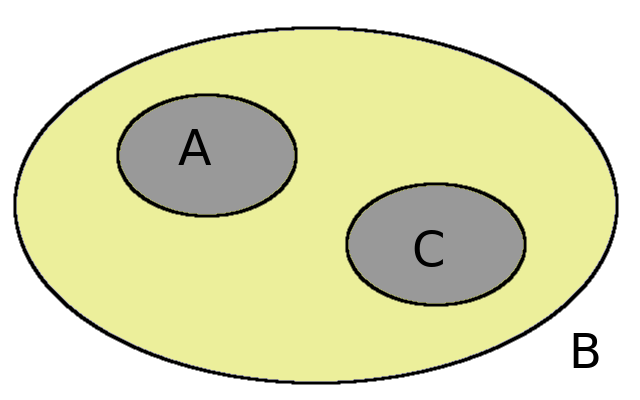
\includegraphics[width=5cm]{exerc3.png}
               
               \end{figure}
 
     \end{minipage}

\item Considere o diagrama abaixo e dê, por extensão, os conjuntos $A$ e $B$

\begin{figure}[H]

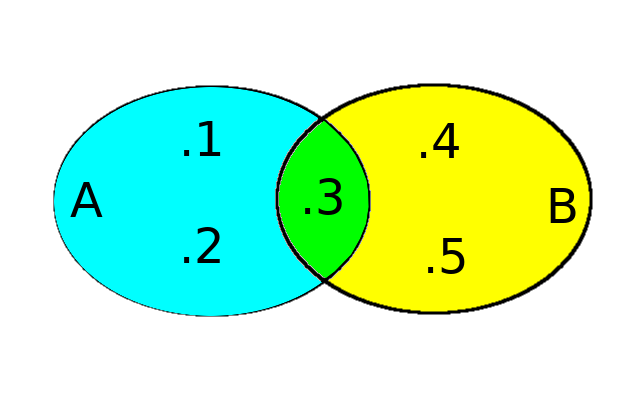
\includegraphics[width=4cm]{exec4.png}

\end{figure}

\item Considere o diagrama abaixo e dê, por extensão, os conjuntos $X$ e $Y$

\begin{figure}[H]

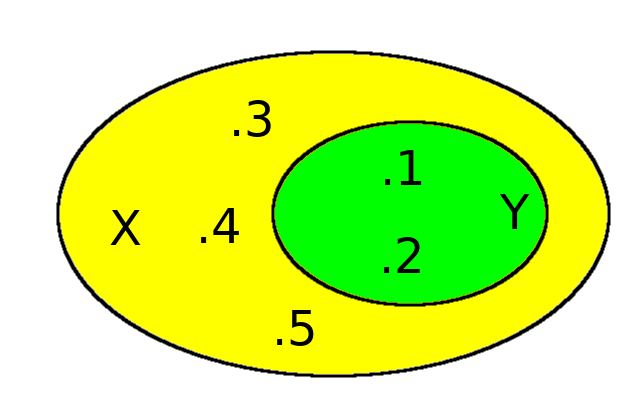
\includegraphics[width=4cm]{exec5.png}

\end{figure}

\item Sendo $A=\{0, 1, 2, 3\}$, $B=\{0, 2, 3, 5\}$, $C=\{x \mid x$ é um número par positivo menor que $10\}$ e $D=\{x \mid x$ é um número ímpar compreendido entre $4$ e $10\}$, determine:

               \begin{enumerate}[label=\textbf{\alph*)}]
               \item $A \cup B$
               \item $A \cup C$
               \item $A \cup D$
               \item $B \cup C$
               \item $B \cup D$
               \item $C \cup D$
               \end{enumerate}

\item Sendo $A=\{0, 1, 2, 3, 4\}$, $B=\{0, 1, 2\}$, $C=\{x \mid s$ é par positivo menor que $10\}$ e $D=\{x \mid x$ é ímpar compreendido entre $0$ e $6\}$, determine:

               \begin{enumerate}[label=\textbf{\alph*)}]
               \item $A \cap B$
               \item $A \cap C$
               \item $C \cap D$
               \item $B \cap C$
               \item $(A \cap B) \cap C$
               \item $(A \cap C) \cap D$
               \end{enumerate}

\item Responda:

               \begin{enumerate}[label=\textbf{\alph*)}]
               \item Se $A \cap B= \emptyset $, como se chamam os conjuntos $A$ e $B$?
               \item Se um conjunto $A$ tem 3 elementos e um conjunto $B$ tem 5 elementos, quantos elementos, no máximo, terá o conjunto $A \cap B$?
               \item Se $A$ e $B$ são disjuntos, quantos elementos terá o conjunto $A \cap B$?
               \end{enumerate}

\item Dados $A=\{0, 1, 2, 3\}$, $B=\{0, 2, 4\}$, $C=\{1, 3, 5\}$ e $D=\{2, 3\}$, determine:

               \begin{enumerate}[label=\textbf{\alph*)}]
               \item $(A \cap B) \cup C$
               \item $(B \cup D) \cap A$
               \item $(A \cup C) \cap D$
               \item $(A \cap B) \cup (C \cap D)$
               \item $(A \cup D) \cap (B \cup C)$
               \item $(A \cap C) \cap (B \cup D)$
               \end{enumerate}
               
\item Sendo $A$ o conjunto dos divisores naturais de $18$ e $B$ o conjunto dos divisores naturais de $30$, escreva:

               \begin{enumerate}[label=\textbf{\alph*)}]
               \item O conjunto $A$.
               \item O conjunto $B$.
               \item O conjunto dos divisores comuns de $18$ e $30$.
               \item O máximo divisor comum de $18$ e $30$.
               \end{enumerate}

\item Considere os  conjuntos $A=\{$divisores naturais de $30\}$, $B=\{$múltiplos de $6\}$ e $C=\{$múltiplos de $3\}$. Calcule:

               \begin{enumerate}[label=\textbf{\alph*)}]
               \item $A \cup C$
               \item $B \cap C$
               \item $A \cap (B \cup C)$
               \item $A \cap B \cap C$
               \item Quais os elementos de $A$ que não pertencem a $B$.
               \end{enumerate}

\item Com base no diagrama ao lado, calcule:

       \begin{minipage}{.3\linewidth}

               \begin{enumerate}[label=\textbf{\alph*)}]
               \item $A \cup B$
               \item $A \cap C$
               \item $A \cup C$
               \item $B \cap C$
               \item $B \cup C$
               \end{enumerate}

       \end{minipage}
       \begin{minipage}{.3\linewidth}
       
               \begin{enumerate}[resume, label=\textbf{\alph*)}]
               \item $A \cap B \cap C$
               \item $A \cup B \cup C$
               \item $(A \cup B) \cap C$
               \item $(A \cap B)$
               \item $(A \cap B) \cup C$
               \end{enumerate}
       
       \end{minipage}
       \begin{minipage}{.3\linewidth}
               \begin{figure}[H]
               
               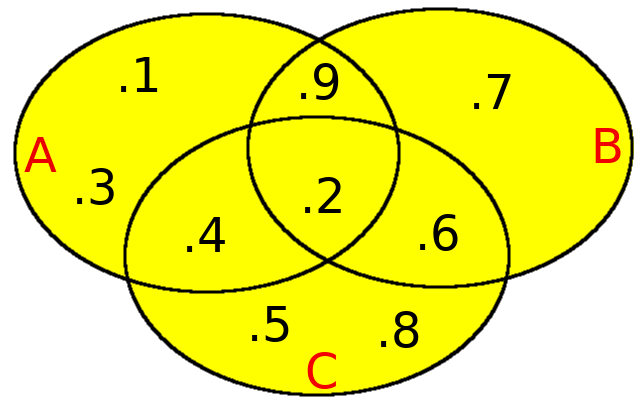
\includegraphics[width=6cm]{exerc6.png}
               
               \end{figure}
       
       \end{minipage}

\item Dados $A=\{0, 1, 2, 3\}$, $B=\{1, 2, 3\}$ e $C=\{2, 3, 4, 5\}$, determine:

       \begin{minipage}{.3\linewidth}
       
                \begin{enumerate}[label=\textbf{\alph*)}]
                \item $A-B$
                \item $A-C$
                \item $B-C$
                \end{enumerate}
       
       \end{minipage}
       \begin{minipage}{.3\linewidth}
       
                \begin{enumerate}[resume, label=\textbf{\alph*)}]
                \item $(A \cap B)-C$
                \item $(A-C) \cap (B-C)$
                \item $A- \emptyset$
                \end{enumerate}
       
       \end{minipage}
       \begin{minipage}{.3\linewidth}

                \begin{enumerate}[resume, label=\textbf{\alph*)}]
                \item $\complement_{A^{B}}$
                \item $\complement_{A^{(B \cap C)}}$
                \item $(\emptyset-B) \cup \complement_{C^{\emptyset}}$
                \end{enumerate}
       
       \end{minipage}
       
\item Diga qual proposição é verdadeira e qual é falsa:

       \begin{minipage}{.4\linewidth}

                \begin{enumerate}[label=\textbf{\alph*)}]
                \item $A \cap \emptyset$
                \item $A- \emptyset$
                \item $\emptyset-A=\emptyset$
                \item $(A-A) \cup A=A$
                \end{enumerate}
       
       \end{minipage}
       \begin{minipage}{.4\linewidth}

                \begin{enumerate}[resume, label=\textbf{\alph*)}]
                \item $(A-A) \cap A=A$
                \item $(A \cap A) \cup \emptyset=\emptyset$
                \item $\complement_{A^{(\complement_{A^{B}})}}=B$ com $B \subset A$
                \end{enumerate}
       
       \end{minipage}

\end{enumerate}

\end{comment}

%\end{comment}

\begin{comment}

\chapter*{Gabarito}

\begin{enumerate}[label=\textbf{\arabic*)}]

\item a) Finito, \hspace{2cm} b) Infinito, \hspace{2cm} c) Vazio

\item a) $A \subset B$, \hspace{2cm} b) $A \subset C$, \hspace{2cm} c)  $B \not\subset C$ 

\item a) V, \hspace{2cm} b) V, \hspace{2cm} c) F, \hspace{2cm} d) F, \hspace{2cm} e) V, 

f) V, \hspace{2cm} g) V, \hspace{2cm} h) V

\item $A=\{1, 2, 3\}$ e $B=\{3, 4, 5\}$
\item $X=\{1, 2, 3, 4, 5\}$ e $Y=\{1, 2\}$
\item a) $\{0, 1, 2, 3, 5\}$, \hspace{2.7cm} b) $\{0, 1, 2, 3, 4, 6, 8\}$, \hspace{1.5cm} c) $\{0, 1, 2, 3, 5, 7, 9\}$, 

d) $\{0, 2, 3, 4, 5, 6, 8 \}$, \hspace{2cm} e) $\{0, 2, 3, 5, 7, 9\}$, \hspace{2cm} f) $\{0, 2, 4, 5, 6, 7, 8, 9\}$
\item a) $\{0, 1, 2\}$, \hspace{2cm} b) $\{0, 2, 4\}$,\hspace{2cm} c) $\{1, 3\}$ 

d) $\{0, 2\}$, \hspace{2.3cm} e) $\{0,2\}$, \hspace{2.3cm} f) $\emptyset$
\item a) disjuntos, \hspace{2cm} b) 3, \hspace{2cm} c) zero
\item a) $\{0, 1, 2, 3, 5\}$, \hspace{2cm} b) $\{0, 2, 3\}$, \hspace{2cm} c) $\{2, 3\}$, 

d) $\{0, 2, 3\}$, \hspace{2.7cm} e) $\{0, 1, 2, 3\}$, \hspace{1.8cm} f) $\{3\}$
\item a) $A=\{1, 2, 3, 5\}$, \hspace{2cm} b) $B=\{1, 2, 3, 5, 6, 10, 15, 30\}$, \hspace{2cm} c) $\{1, 2, 3, 6\}$,\hspace{2cm} d) $6$.
\item a) $\{3, 6, 15, 30\}$,\hspace{2cm} b) $B$, \hspace{2cm} c) $\{3, 6, 15, 30\}$, 

d) $\{6, 30\}$, \hspace{2.7cm} e) $\{1, 2, 3, 5, 10, 15\}$
\item a) $\{1, 2, 3, 4, 6, 7, 9\}$,\hspace{1.5cm} b) $\{2, 4\}$, \hspace{4cm} c) $\{1 , 2, 3, 4, 5, 6, 8, 9\}$, 

d) $\{2, 6\}$ \hspace{3.3cm} e) $\{2, 4, 5, 6, 7, 8, 9\}$, \hspace{2.2cm} f) $\{2\}$, 

g) $\{1, 2, 3, 4, 5, 6, 7, 8, 9\}$, \hspace{.7cm} h) $\{2, 4, 6\}$, \hspace{3.6cm} i) $\{2, 9\}$,

 j) $\{2, 4, 5, 6, 8, 9\}$
\item a) $\{0\}$, \hspace{2cm} b) $\{0, 1\}$, \hspace{2cm} c) $\{1\}$, \hspace{2cm}d) $\{1\}$, 

e) $\{1\}$, \hspace{2cm} f) $\{0, 1, 2, 3\}$, \hspace{1.4cm} g) $\{0\}$, \hspace{1.8cm} h) $\{0, 1\}$, 

i) $\{2, 3, 4, 5\}$

\item a) V, \hspace{2cm}b) V, \hspace{2cm} c) V, \hspace{2cm} d) V, \hspace{2cm} e) F, 

f) F, \hspace{2cm} g) V
\end{enumerate}

\end{comment}

\end{SingleSpace}

\end{document}